%----------------------------------------------------------------------------------------
%	PACKAGES AND OTHER DOCUMENT CONFIGURATIONS
%----------------------------------------------------------------------------------------

\documentclass{article}

\usepackage{fancyhdr} % Required for custom headers
\usepackage{lastpage} % Required to determine the last page for the footer
\usepackage{extramarks} % Required for headers and footers
\usepackage[usenames,dvipsnames]{color} % Required for custom colors
\usepackage{pgf} % Required to insert pgf plots from matplotlib
\usepackage{graphicx} % Required to insert images
\usepackage{listings} % Required for insertion of code
\usepackage{courier} % Required for the courier font
\usepackage{lipsum} % Used for inserting dummy 'Lorem ipsum' text into the template
\usepackage[utf8]{inputenc}
\usepackage[ngerman]{babel}
\usepackage{subcaption, caption, tabularx, minted}
\usepackage{hyperref}

% Margins
\topmargin=-0.45in
\evensidemargin=0in
\oddsidemargin=0in
\textwidth=6.5in
\textheight=9.0in
\headsep=0.25in

\linespread{1.1} % Line spacing

% Set up the header and footer
\pagestyle{fancy}
%\lhead{\hmwkAuthorName} % Top left header
\chead{\hmwkClass\ : \hmwkTitle} % Top center head
\rhead{\firstxmark} % Top right header
\lfoot{\lastxmark} % Bottom left footer
\cfoot{} % Bottom center footer
\rfoot{Page\ \thepage\ of\ \protect\pageref{LastPage}} % Bottom right footer
\renewcommand\headrulewidth{0.4pt} % Size of the header rule
\renewcommand\footrulewidth{0.4pt} % Size of the footer rule

\setlength\parindent{0pt} % Removes all indentation from paragraphs

%----------------------------------------------------------------------------------------
%	CODE INCLUSION CONFIGURATION
%----------------------------------------------------------------------------------------

\definecolor{MyDarkGreen}{rgb}{0.0,0.4,0.0} % This is the color used for comments
\lstloadlanguages{Perl} % Load Perl syntax for listings, for a list of other languages supported see: ftp://ftp.tex.ac.uk/tex-archive/macros/latex/contrib/listings/listings.pdf
\lstset{language=Perl, % Use Perl in this example
        frame=single, % Single frame around code
        basicstyle=\small\ttfamily, % Use small true type font
        keywordstyle=[1]\color{Blue}\bf, % Perl functions bold and blue
        keywordstyle=[2]\color{Purple}, % Perl function arguments purple
        keywordstyle=[3]\color{Blue}\underbar, % Custom functions underlined and blue
        identifierstyle=, % Nothing special about identifiers                                         
        commentstyle=\usefont{T1}{pcr}{m}{sl}\color{MyDarkGreen}\small, % Comments small dark green courier font
        stringstyle=\color{Purple}, % Strings are purple
        showstringspaces=false, % Don't put marks in string spaces
        tabsize=5, % 5 spaces per tab
        %
        % Put standard Perl functions not included in the default language here
        morekeywords={rand},
        %
        % Put Perl function parameters here
        morekeywords=[2]{on, off, interp},
        %
        % Put user defined functions here
        morekeywords=[3]{test},
       	%
        morecomment=[l][\color{Blue}]{...}, % Line continuation (...) like blue comment
        numbers=left, % Line numbers on left
        firstnumber=1, % Line numbers start with line 1
        numberstyle=\tiny\color{Blue}, % Line numbers are blue and small
        stepnumber=5 % Line numbers go in steps of 5
}

% Creates a new command to include a perl script, the first parameter is the filename of the script (without .pl), the second parameter is the caption
\newcommand{\perlscript}[2]{
\begin{itemize}
\item[]\lstinputlisting[caption=#2,label=#1]{#1.pl}
\end{itemize}
}

%----------------------------------------------------------------------------------------
%	DOCUMENT STRUCTURE COMMANDS
%	Skip this unless you know what you're doing
%----------------------------------------------------------------------------------------

% Header and footer for when a page split occurs within a problem environment
\newcommand{\enterProblemHeader}[1]{
%\nobreak\extramarks{#1}{#1 continued on next page\ldots}\nobreak
%\nobreak\extramarks{#1 (continued)}{#1 continued on next page\ldots}\nobreak
}

% Header and footer for when a page split occurs between problem environments
\newcommand{\exitProblemHeader}[1]{
%\nobreak\extramarks{#1 (continued)}{#1 continued on next page\ldots}\nobreak
%\nobreak\extramarks{#1}{}\nobreak
}

\setcounter{secnumdepth}{0} % Removes default section numbers
\newcounter{homeworkProblemCounter} % Creates a counter to keep track of the number of problems

\newcommand{\homeworkProblemName}{}
\newenvironment{homeworkProblem}[1][Problem \arabic{homeworkProblemCounter}]{ % Makes a new environment called homeworkProblem which takes 1 argument (custom name) but the default is "Problem #"
\stepcounter{homeworkProblemCounter} % Increase counter for number of problems
\renewcommand{\homeworkProblemName}{#1} % Assign \homeworkProblemName the name of the problem
\section{\homeworkProblemName} % Make a section in the document with the custom problem count
%\enterProblemHeader{\homeworkProblemName} % Header and footer within the environment
}{
%\exitProblemHeader{\homeworkProblemName} % Header and footer after the environment
}

\newcommand{\problemAnswer}[1]{ % Defines the problem answer command with the content as the only argument
\noindent\framebox[\columnwidth][c]{\begin{minipage}{0.98\columnwidth}#1\end{minipage}} % Makes the box around the problem answer and puts the content inside
}

\newcommand{\homeworkSectionName}{}
\newenvironment{homeworkSection}[1]{ % New environment for sections within homework problems, takes 1 argument - the name of the section
\renewcommand{\homeworkSectionName}{#1} % Assign \homeworkSectionName to the name of the section from the environment argument
\subsection{\homeworkSectionName} % Make a subsection with the custom name of the subsection
%\enterProblemHeader{\homeworkProblemName\ [\homeworkSectionName]} % Header and footer within the environment
}{
%\enterProblemHeader{\homeworkProblemName} % Header and footer after the environment
}

%----------------------------------------------------------------------------------------
%	NAME AND CLASS SECTION
%----------------------------------------------------------------------------------------

\newcommand{\hmwkTitle}{Exercise\ \#7} % Assignment title
\newcommand{\hmwkDueDate}{Tuesday,\ June 9,\ 2015} % Due date
\newcommand{\hmwkClass}{Advanced Parallel Computing} % Course/class
\newcommand{\hmwkClassTime}{} % Class/lecture time
\newcommand{\hmwkClassInstructor}{} % Teacher/lecturer
\newcommand{\hmwkAuthorName}{Svend Dorkenwald, Günther Schindler} % Your name

%----------------------------------------------------------------------------------------
%	TITLE PAGE
%----------------------------------------------------------------------------------------

\title{
\vspace{2in}
\textmd{\textbf{\hmwkClass:\ \hmwkTitle}}\\
\normalsize\vspace{0.1in}\small{Due\ on\ \hmwkDueDate}\\
\vspace{0.1in}\large{\textit{\hmwkClassTime}}
\vspace{3in}
}

\author{\textbf{\hmwkAuthorName}}
\date{} % Insert date here if you want it to appear below your name

%----------------------------------------------------------------------------------------

\begin{document}

\maketitle

%----------------------------------------------------------------------------------------
%	TABLE OF CONTENTS
%----------------------------------------------------------------------------------------

%\setcounter{tocdepth}{1} % Uncomment this line if you don't want subsections listed in the ToC

\newpage
%\tableofcontents
\newpage

%----------------------------------------------------------------------------------------
%	Reading
%----------------------------------------------------------------------------------------

\begin{homeworkProblem}[Reading]
\subsection{Why the grass may not be greener on the other side: a comparison of locking vs. transactional memory}
McKenney et. al discuss the strength and weaknesses of locking and transactional memory schemes. They analyse those and give suggestions for further improvement. \\
Their work shows that locking solutions might not be perfectly suited, but since it is widely used many workarounds were developed for certain problems. Transactional memory on the other side might look like very elegant at first glance, but leads to many ugly problems. Moreover, a large community working on these problems is missing. The authors do not doom TM to the bin, but argue that it need to focus on applications which preexisting machanisms poorly serve to grow a support. \\
Surprisingly, this paper might be mostly correct today showing how little progress was reached in the last two decades. Both schemes might have improved since then, but few of their main problems are overcome - even their supposed remaining challenges for locking are still not solved today. We give this paper a strong accept.



\subsection{Stretching transactional memory}
Dragojevic, Guerraoui and Kapalka present their Software Transactional Memory implementation (Swiss TM). To proof that Swiss TM is superior to other implementations they compare their performances in different benchmarks. \\
The key asset of their implementation is their two-phase contention manager. Unlike other STMs they use eager and lazy strategy. SwissTM  detects write/write conflicts eagerly and read/write conflicts lazily. This makes it effective for mixed workloads containing non-uniform, dnyamic data structures and various transaction sizes. \\
We like the way the authors try to improve existing schemes by combining different strategies to use them at what they are best. However, it remains unclear how their implementation stacks up against HTM or even current Mutex implementations. If STM should be the standard one day they have to compete with currently used systems, otherwise their work is only meant to be recognized by a small community. Additionaly, they name problems like that their implementation is not privatization-safe which ''did not affect us (they), as none of the benchmarks we (they) use requires privatization-safe ST''. \\
Nevertheless, we give this paper a weak accept.

\end{homeworkProblem}

%----------------------------------------------------------------------------------------
%	Red-Black Tree – Implementation of sequential version
%----------------------------------------------------------------------------------------

\begin{homeworkProblem}[Red-Black Tree – Implementation of sequential version]
Our red-black tree will implement an associative array, so we will store both the key 
and its associated value. 
\begin{lstlisting}{c}
typedef struct rbtree_node_t {
    void* key;
    void* value;
    struct rbtree_node_t* left;
    struct rbtree_node_t* right;
    struct rbtree_node_t* parent;
    enum rbtree_node_color color;
} *rbtree_node;
\end{lstlisting}
Each node also stores its color, either red or black, using an enumeration.
\\\\
We will at all times enforce the following five properties, which provide a theoretical 
guarantee that the tree remains balanced. 
\begin{itemize}
\item Each node is either red or black
\item The root node is black
\item All leaves are black and contain no data
\item Every red node has two children, and both are black
\item All paths from any given node to its leaf nodes contain the same number of black 
nodes
\end{itemize}
We will have a helper function
\begin{lstlisting}{c}
void verify_properties(rbtree t)
\end{lstlisting}
that asserts all five properties in a debug build, to help verify the correctness of 
our implementation.
\\\\
An empty tree is represented by a tree with a NULL root. The function 
\begin{lstlisting}{c}
rbtree rbtree_create()
\end{lstlisting}
provides a starting point for other operations.
\\\\
Searching for values is straightforward, by finding the node and extracting the data if 
lookup succeeded.
\begin{lstlisting}{c}
void* rbtree_lookup(rbtree t, void* key, compare_func compare);
\end{lstlisting}
We return NULL if the key was not found.
\\\\
When inserting a new value, we first insert it into the tree as we would into an 
ordinary binary search tree. If the key already exists, we just replace the value.
\begin{lstlisting}{c}
void rbtree_insert(rbtree t, void* key, void* value, compare_func compare)
\end{lstlisting}
Otherwise, we find the place in the tree where the new pair belongs, then attach a
newly created red node containing the value.

\end{homeworkProblem}

%----------------------------------------------------------------------------------------
%	Red-Black Tree – Sequential Performance
%----------------------------------------------------------------------------------------

\begin{homeworkProblem}[Red-Black Tree – Sequential Performance]
Since the searching and inserting time is ${\mathcal O(log (n))}$, where n is the total 
number of elements (constant 10M) in the tree, we expect constant OPS for different 
lengths of the update stream.
\begin{center}
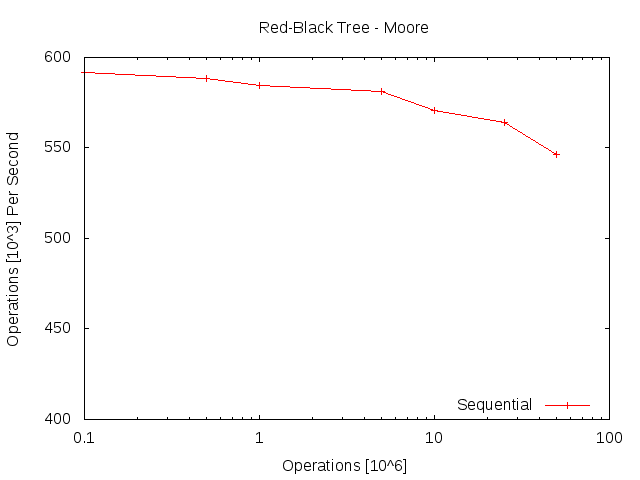
\includegraphics[width=0.7\columnwidth]{update_rate.png}
\end{center}
As the graphic shows, we actually get a almost constant number of OPS for the sequential
Red-Black Tree.
\end{homeworkProblem}

\clearpage
\end{document}
